\newpage
\chapter{Proposed Methodology}

\section{System Architecture}
The implemented architecture adheres to a clean, decoupled three-tier pattern. This section details the internal mechanics of each layer.

\subsection{Client-Side Architecture (React 18 + Vite)}
The user interface is engineered using React 18, bundled using the Vite build tool. The client features:
\begin{itemize}
    \item \textbf{Declarative Routing:} Powered by \texttt{react-router-dom} v6, managing nested routes, private authenticated dashboard paths protected by \texttt{ProtectedRoute.jsx}, and dynamic URL parameter lookups.
    \item \textbf{Global Context Providers:}
    \begin{itemize}
        \item \texttt{AuthContext.jsx}: Centralizes user login credentials, JWT tokens in \texttt{localStorage}, and role authorization flags.
        \item \texttt{ToastContext.jsx}: Delivers non-intrusive floating feedback alerts for asynchronous operations.
    \end{itemize}
    \item \textbf{Axios HTTP Interceptors:} Automatically injects the \texttt{Authorization: Bearer <token>} header into every outgoing request and intercepts 401 Unauthorized responses to perform clean session logouts.
\end{itemize}

\subsection{Server-Side REST API Architecture (Node.js + Express.js)}
The server gateway operates on top of Node.js 24 and Express 4.19:
\begin{itemize}
    \item \textbf{Security Middleware:} Helmet secures HTTP response headers (XSS filter, frameguard, noSniff); CORS enforces origin whitelisting across allowed frontend development and production hosts.
    \item \textbf{Response Standardization:} All API endpoints return a standardized envelope structure via \texttt{ApiResponse.js}:
    \begin{equation}
    \text{Response} = \{ \text{success: boolean}, \text{message: string}, \text{data: object/array}, \text{timestamp: ISO8601} \}
    \end{equation}
    \item \textbf{Pagination Utility:} Emulates the Spring Data \texttt{Page<T>} contract (\texttt{content}, \texttt{totalElements}, \texttt{totalPages}, \texttt{size}, \texttt{number}), guaranteeing zero breaking changes on the frontend UI.
\end{itemize}

\section{Security Architecture \& RBAC Implementation}
Authentication and role authorization are enforced through stateless cryptographic mechanisms:
\begin{enumerate}
    \item \textbf{Password Security:} User passwords are encrypted prior to persistence using \texttt{bcryptjs} with an adaptive cost factor of 10 salt rounds:
    \begin{equation}
    \text{Hash} = \operatorname{Bcrypt}(\text{password}, \operatorname{Salt}(10))
    \end{equation}
    \item \textbf{JWT Generation \& Verification:} Upon successful login, the server issues a signed HMAC-SHA256 JWT payload containing user ID, email, and roles with an expiration of 24 hours (86,400,000 ms).
    \item \textbf{RBAC Middleware (\texttt{rbac.js}):} Provides higher-order route guards:
    \begin{itemize}
        \item \texttt{hasRole(roleName)}: Ensures the user possesses the exact required authority.
        \item \texttt{hasAnyRole([...])}: Authorizes requests if the user possesses at least one matching role from the authorized list.
    \end{itemize}
\end{enumerate}

\begin{table}[h!]
\centering
\caption{Role-Based Access Control (RBAC) Permission Matrix}\label{tab:rbac_matrix}
\begin{tabular}{|l|c|c|c|c|c|}
\hline
\textbf{Endpoint / Operation} & \textbf{Admin} & \textbf{Employer} & \textbf{Worker} & \textbf{Customer} & \textbf{Provider} \\ \hline
\texttt{GET /api/v1/jobs} & \checkmark & \checkmark & \checkmark & \checkmark & \checkmark \\ \hline
\texttt{POST /api/v1/jobs} & $\times$ & \checkmark & $\times$ & $\times$ & $\times$ \\ \hline
\texttt{POST /api/v1/jobs/:id/apply} & $\times$ & $\times$ & \checkmark & $\times$ & $\times$ \\ \hline
\texttt{PUT /jobs/applications/:id/status} & $\times$ & \checkmark & $\times$ & $\times$ & $\times$ \\ \hline
\texttt{POST /api/v1/requests} & $\times$ & $\times$ & $\times$ & \checkmark & $\times$ \\ \hline
\texttt{PUT /requests/:id/status} & $\times$ & $\times$ & $\times$ & $\times$ & \checkmark \\ \hline
\texttt{POST /api/v1/reviews} & \checkmark & \checkmark & \checkmark & \checkmark & \checkmark \\ \hline
\texttt{POST /api/v1/complaints} & \checkmark & \checkmark & \checkmark & \checkmark & \checkmark \\ \hline
\texttt{GET /api/v1/admin/*} & \checkmark & $\times$ & $\times$ & $\times$ & $\times$ \\ \hline
\texttt{POST /api/v1/categories} & \checkmark & $\times$ & $\times$ & $\times$ & $\times$ \\ \hline
\end{tabular}
\end{table}

\section{Database Design \& MongoDB Schema Collections}
Data persistence is structured across 15 collections in MongoDB Atlas:
\begin{enumerate}
    \item \textbf{\texttt{users}:} Stores core authentication identity, roles array, and suspension status.
    \item \textbf{\texttt{roles}:} Role definitions (\texttt{ROLE\_ADMIN}, \texttt{ROLE\_EMPLOYER}, \texttt{ROLE\_WORKER}, etc.).
    \item \textbf{\texttt{skills}:} Master taxonomy of 14 trade and employment skills.
    \item \textbf{\texttt{servicecategories}:} Master directory of 6 on-demand trade categories.
    \item \textbf{\texttt{workerprofiles}:} Stores worker bio, trade skills array, daily/hourly rates, and availability.
    \item \textbf{\texttt{employerprofiles}:} Stores business information, company name, contact person, and address.
    \item \textbf{\texttt{customerprofiles}:} Stores customer service delivery address and coordinates.
    \item \textbf{\texttt{providerprofiles}:} Stores contractor pricing, trade license ID proof, and verification status.
    \item \textbf{\texttt{jobs}:} Stores employer job postings, wage type, salary range, and required skill IDs.
    \item \textbf{\texttt{jobapplications}:} Stores candidate applications, wage bids, cover notes, and status.
    \item \textbf{\texttt{servicerequests}:} Stores on-demand service bookings, scheduled dates, and 5-step status.
    \item \textbf{\texttt{reviews}:} Stores 1-to-5 star ratings and textual reviews linked to users and bookings.
    \item \textbf{\texttt{complaints}:} Stores filed dispute tickets and administrative resolution notes.
    \item \textbf{\texttt{auditlogs}:} Stores tamper-proof platform audit events with user ID, IP, and timestamp.
    \item \textbf{\texttt{counters}:} Dedicated sequence counter collection maintaining atomic increments.
\end{enumerate}

\subsection{Atomic Sequence Generator Implementation}
Because the frontend contracts rely on numeric identifiers (e.g. \texttt{jobId: 1, 2}), a dedicated atomic counter generator is utilized:
\begin{equation}
\operatorname{getNextId}(\text{sequenceName}) \implies \operatorname{findOneAndUpdate}(\{ \text{\_id}: \text{sequenceName} \}, \{ \$inc: \{ \text{seq}: 1 \} \}, \{ \text{new}: \text{true}, \text{upsert}: \text{true} \})
\end{equation}
This guarantees thread-safe, strictly monotonic unique integer identifiers without collision risks.

\section{Implementation Approach}
The development methodology followed an agile, test-driven approach:
\begin{enumerate}
    \item \textbf{Schema Modeling:} Defined Mongoose schemas matching the relational entities with strict validation rules.
    \item \textbf{Controller \& Route Implementation:} Implemented business controllers and mapped routes according to REST specifications.
    \item \textbf{Database Seeding:} Formulated \texttt{seedData.js} to pre-populate all master reference data and five test user accounts.
    \item \textbf{Automated Test Engineering:} Authored 16 automated integration tests using the native Node.js test runner and Supertest.
    \item \textbf{Cloud Deployment Pipeline:} Established automated Git hooks deploying to Render and Vercel.
\end{enumerate}

\section{System User Interface and Website Screenshots}
The user interface of Labour Connect is designed with a modern, responsive layout prioritizing accessibility for daily-wage workers, employers, customers, and trade technicians. The system is deployed and accessible live at \url{https://labour-connect-updated.vercel.app/}. Figures~\ref{fig:screenshot_landing} through \ref{fig:screenshot_deployment} display the primary operational views of the production application.

\subsection{Landing and Discovery Interface}
Figure~\ref{fig:screenshot_landing} depicts the landing page of Labour Connect, presenting the platform's dual operational verticals: the skilled daily-wage employment marketplace and on-demand hyperlocal trade bookings.

\begin{figure}[h!]
\centering
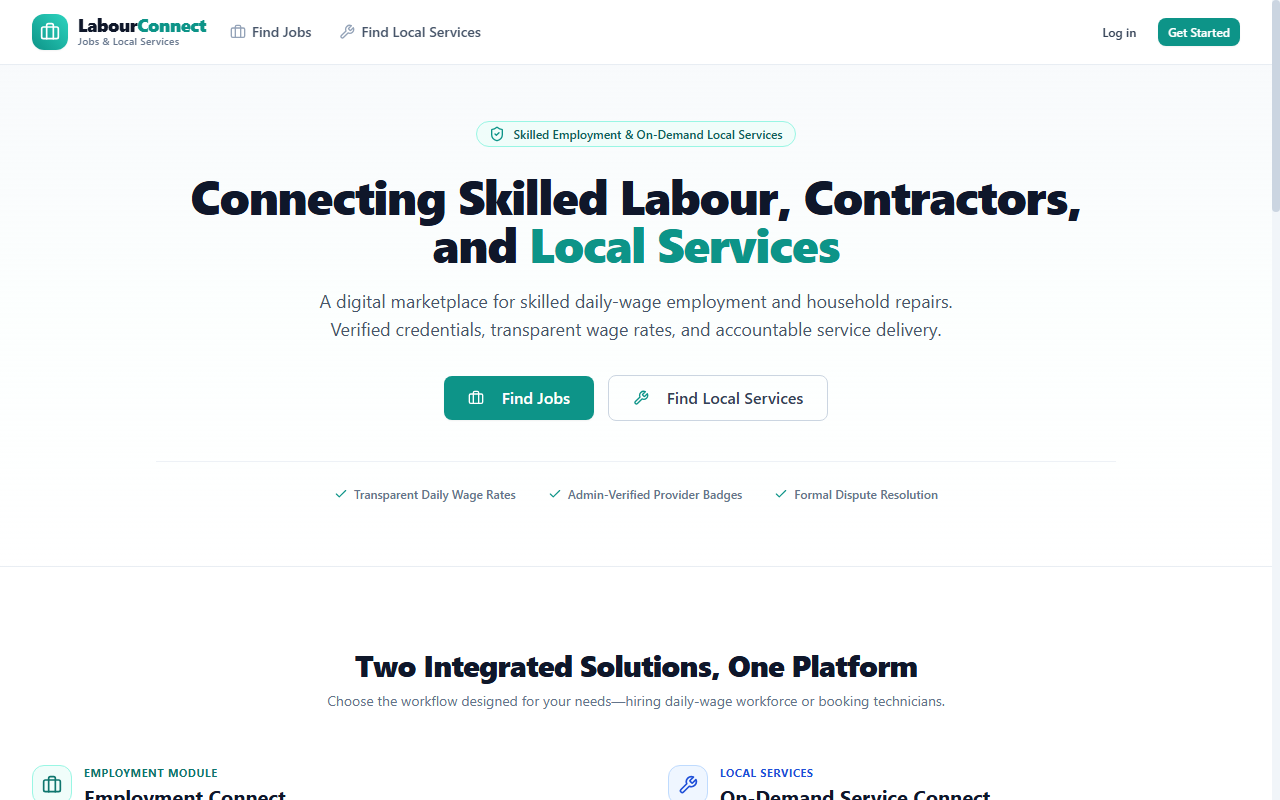
\includegraphics[width=0.92\textwidth]{screenshot_landing}
\caption{Labour Connect Landing Interface featuring Dual Operational Portals}\label{fig:screenshot_landing}
\end{figure}

\subsection{Skilled Jobs Marketplace}
Figure~\ref{fig:screenshot_jobs} shows the public job browsing and filtering module, allowing workers to search vacancies by trade category, employment model (daily-wage or monthly), and wage threshold.

\begin{figure}[h!]
\centering
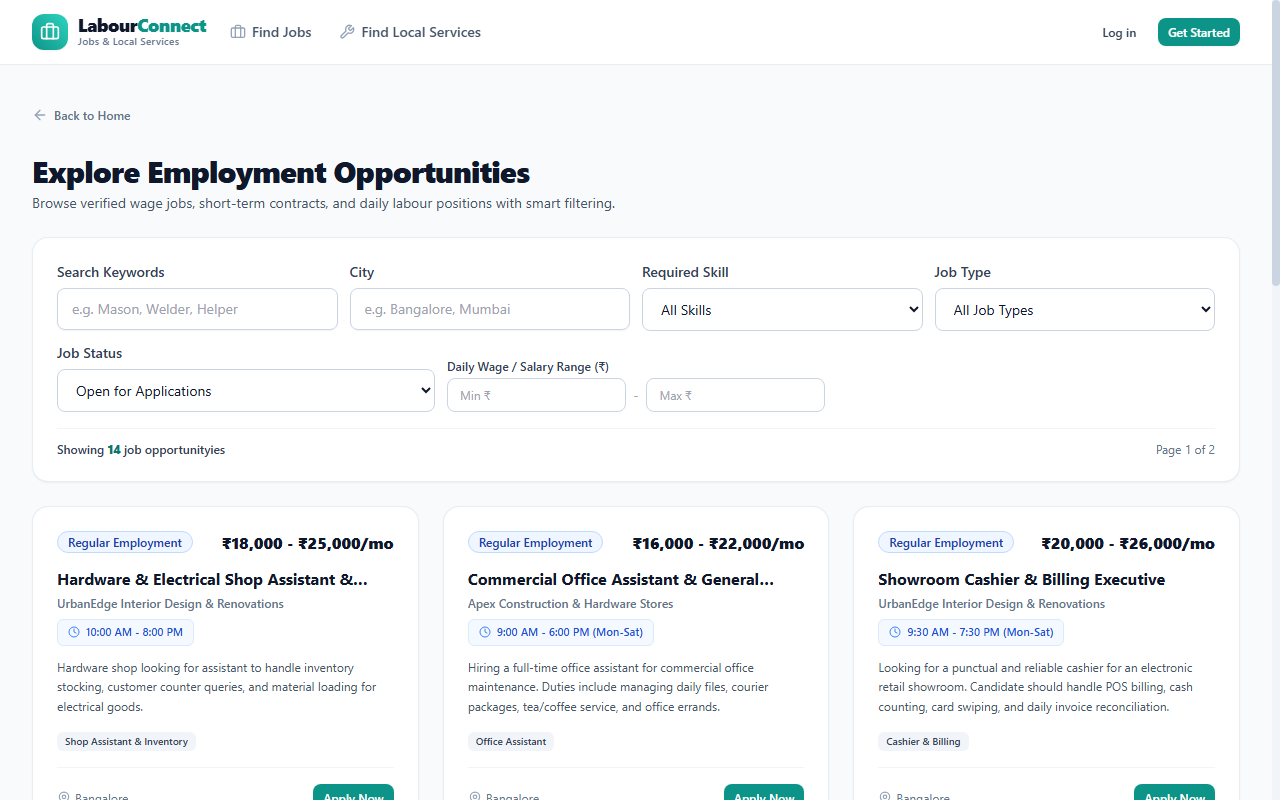
\includegraphics[width=0.92\textwidth]{screenshot_jobs}
\caption{Skilled Employment Marketplace with Real-Time Filtering and Wage Transparency}\label{fig:screenshot_jobs}
\end{figure}

\subsection{On-Demand Hyperlocal Services Directory}
Figure~\ref{fig:screenshot_services} displays the verified service provider discovery page, enabling customers to locate certified technicians filtered by trade category and proximity.

\begin{figure}[h!]
\centering
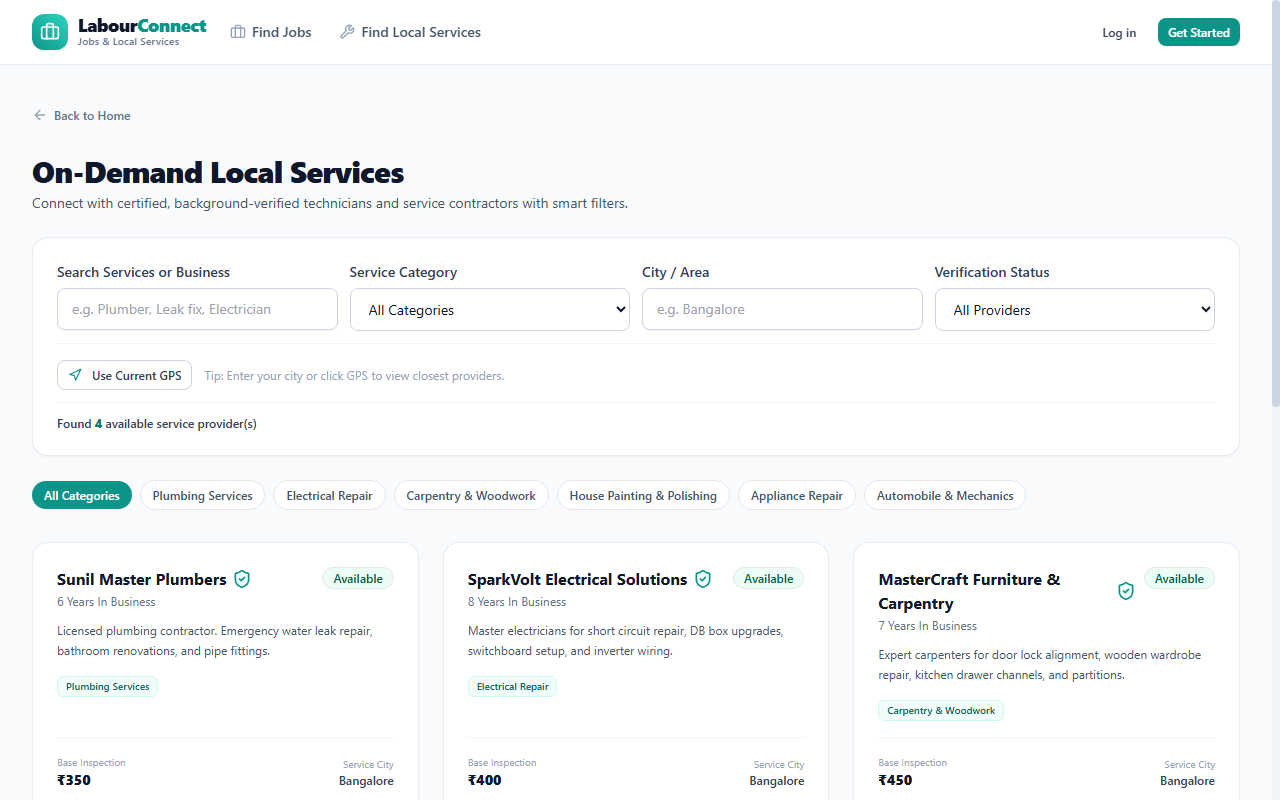
\includegraphics[width=0.92\textwidth]{screenshot_services}
\caption{On-Demand Hyperlocal Service Directory and Verified Provider Catalog}\label{fig:screenshot_services}
\end{figure}

\subsection{Secure Authentication and Role Selection}
Figure~\ref{fig:screenshot_login} illustrates the centralized authentication interface implementing JWT stateless sessions and role-based access delegation.

\begin{figure}[h!]
\centering
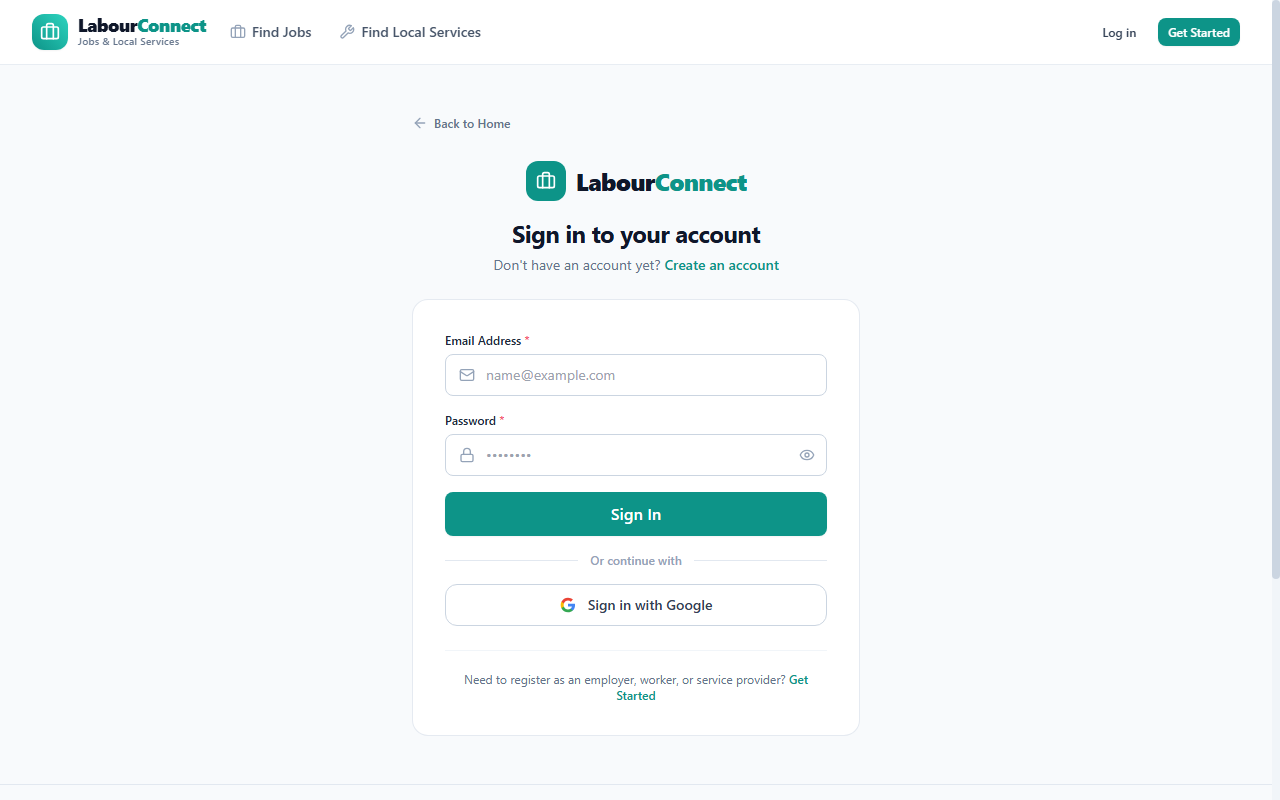
\includegraphics[width=0.75\textwidth]{screenshot_login}
\caption{Authentication Portal Supporting Role-Based Security Governance}\label{fig:screenshot_login}
\end{figure}

\subsection{Production Cloud Deployment}
Figure~\ref{fig:screenshot_deployment} demonstrates the successful production deployment of the client tier on Vercel Global Edge Network connected with Render REST API and MongoDB Atlas.

\begin{figure}[h!]
\centering
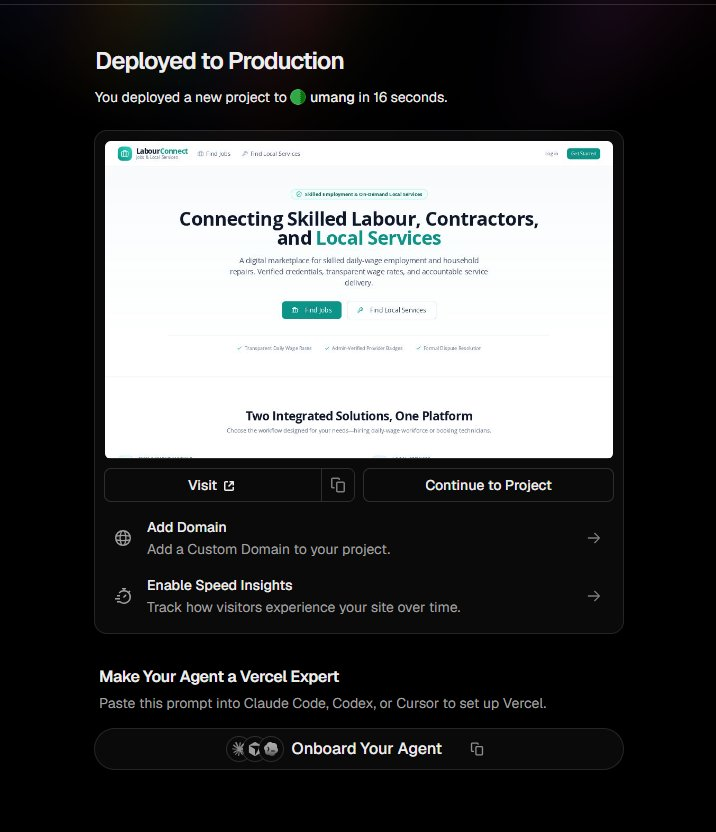
\includegraphics[width=0.88\textwidth]{screenshot_deployment}
\caption{Production Deployment on Vercel Global Edge CDN Infrastructure}\label{fig:screenshot_deployment}
\end{figure}

\vspace{5mm}
\hrule
